\documentclass[border=10pt]{standalone}
\usepackage{tikz}

\begin{document}




\tikzset{every picture/.style={line width=0.75pt}} %set default line width to 0.75pt        

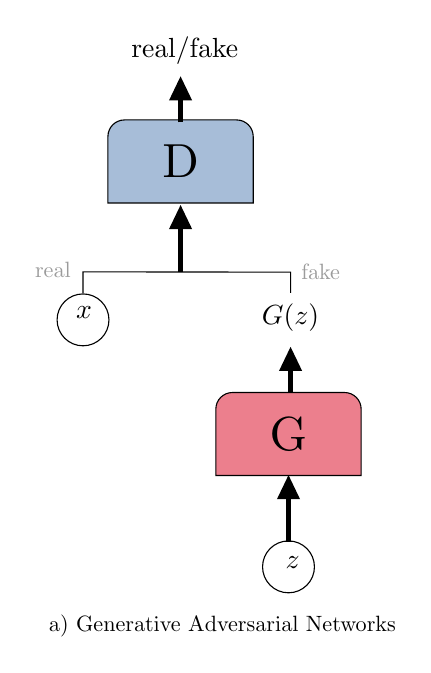
\begin{tikzpicture}[x=0.75pt,y=0.75pt,yscale=-1,xscale=1]
    %uncomment if require: \path (0,300); %set diagram left start at 0, and has height of 300

    %Rounded Same Side Corner Rect [id:dp2451362198380881] 
    \draw  [fill={rgb, 255:red, 167; green, 189; blue, 216 }  ,fill opacity=1 ] (79,54.17) .. controls (79,49.75) and (82.58,46.17) .. (87,46.17) -- (141,46.17) .. controls (145.42,46.17) and (149,49.75) .. (149,54.17) -- (149,86.17) .. controls (149,86.17) and (149,86.17) .. (149,86.17) -- (79,86.17) .. controls (79,86.17) and (79,86.17) .. (79,86.17) -- cycle ;

    %Straight Lines [id:da14573772274169616] 
    \draw [line width=1.5]    (114,47.37) -- (114,28.17) ;
    \draw [shift={(114,25.17)}, rotate = 450] [fill={rgb, 255:red, 0; green, 0; blue, 0 }  ][line width=1.5]  [draw opacity=0] (11.61,-5.58) -- (0,0) -- (11.61,5.58) -- cycle    ;

    %Straight Lines [id:da7579961352080994] 
    \draw [line width=1.5]    (114,109.37) -- (114,90.17) ;
    \draw [shift={(114,87.17)}, rotate = 450] [fill={rgb, 255:red, 0; green, 0; blue, 0 }  ][line width=1.5]  [draw opacity=0] (11.61,-5.58) -- (0,0) -- (11.61,5.58) -- cycle    ;


    %Rounded Same Side Corner Rect [id:dp27437364893503646] 
    \draw  [fill={rgb, 255:red, 236; green, 127; blue, 141 }  ,fill opacity=1 ] (131,185.5) .. controls (131,181.08) and (134.58,177.5) .. (139,177.5) -- (193,177.5) .. controls (197.42,177.5) and (201,181.08) .. (201,185.5) -- (201,217.5) .. controls (201,217.5) and (201,217.5) .. (201,217.5) -- (131,217.5) .. controls (131,217.5) and (131,217.5) .. (131,217.5) -- cycle ;

    %Shape: Circle [id:dp6172800122901183] 
    \draw   (153.5,261.5) .. controls (153.5,254.6) and (159.1,249) .. (166,249) .. controls (172.9,249) and (178.5,254.6) .. (178.5,261.5) .. controls (178.5,268.4) and (172.9,274) .. (166,274) .. controls (159.1,274) and (153.5,268.4) .. (153.5,261.5) -- cycle ;

    %Straight Lines [id:da8111485597522028] 
    \draw    (67,129.5) -- (67,119.37) -- (167,119.5) -- (167,129.5) ;


    %Shape: Circle [id:dp5550396643085889] 
    \draw   (54.5,142.5) .. controls (54.5,135.6) and (60.1,130) .. (67,130) .. controls (73.9,130) and (79.5,135.6) .. (79.5,142.5) .. controls (79.5,149.4) and (73.9,155) .. (67,155) .. controls (60.1,155) and (54.5,149.4) .. (54.5,142.5) -- cycle ;

    %Straight Lines [id:da4358037156768244] 
    \draw [line width=1.5]    (167,177.7) -- (167,158.5) ;
    \draw [shift={(167,155.5)}, rotate = 450] [fill={rgb, 255:red, 0; green, 0; blue, 0 }  ][line width=1.5]  [draw opacity=0] (11.61,-5.58) -- (0,0) -- (11.61,5.58) -- cycle    ;

    %Straight Lines [id:da35373187835236874] 
    \draw [line width=1.5]    (114,109.37) -- (114,119.37) ;


    %Straight Lines [id:da1620841210006193] 
    \draw [line width=1.5]    (166,239.5) -- (166,220.3) ;
    \draw [shift={(166,217.3)}, rotate = 450] [fill={rgb, 255:red, 0; green, 0; blue, 0 }  ][line width=1.5]  [draw opacity=0] (11.61,-5.58) -- (0,0) -- (11.61,5.58) -- cycle    ;

    %Straight Lines [id:da9258346349543058] 
    \draw [line width=1.5]    (166,239.5) -- (166,249.5) ;


    % Text Node
    \draw (167,141.5) node   {$G( z)$};
    % Text Node
    \draw (181.5,119.5) node [scale=0.8,color={rgb, 255:red, 155; green, 155; blue, 155 }  ,opacity=1 ] [align=left] {fake};
    % Text Node
    \draw (52.5,118.5) node [scale=0.8,color={rgb, 255:red, 155; green, 155; blue, 155 }  ,opacity=1 ] [align=left] {real};
    % Text Node
    \draw (116,12.83) node  [align=left] {real/fake};
    % Text Node
    \draw (134.17,290) node [scale=0.8] [align=left] {a) Generative Adversarial Networks};
    % Text Node
    \draw (67.5,139) node   {$x$};
    % Text Node
    \draw (168,259.5) node   {$z$};
    % Text Node
    \draw (166,197.5) node [scale=1.7280000000000002] [align=left] {G};
    % Text Node
    \draw (114,66.17) node [scale=1.7280000000000002] [align=left] {D};


\end{tikzpicture}



\end{document}
